\chapter{Kompressionsalgorithmen}

\section{(exakte) LZ77-Kompression}
Der im Folgenden beschriebene Algorithmus für die Generierung einer exakten LZ77-Faktorisierung dient als Referenz für die Evaluation der approximativen Algorithmen.

\subsection{Konzept}
Wie bereits in Kapitel 2.2 beschrieben, erzeugen Algorithmen der LZ77 - Familie eine Faktorisierung einer Eingabezeichenfolge $S$, wobei die Faktoren entweder Referenzen
zu vorherigen Zeichenfolgen oder einzelne Zeichen sein können. Im Rahmen der exakten LZ77 - Faktorisierung wird ein Greedy - Ansatz verwendet, um von links nach rechts 
stets die längste Zeichenfolge zu referenzieren, die bereits links von der aktuellen Position vorkommt.
\begin{algorithm}[ht]
\centering
\caption{COMP$_{LZ77}$: Exakte LZ77-Faktorisierung mithilfe des Suffix-Arrays} \label{alg:complz77}
\algorithmicrequire $S=e_1...e_n$
\algorithmicensure $F=f_1...f_z$
\begin{algorithmic} [1]
    \STATE $SA \gets SuffixArray(S)$
    \STATE $(NSV, PSV) \gets (NSVArray(S, SA), PSVArray(S, SA))$
    \STATE $F \gets \emptyset$
    \STATE $k \gets 1$
    \WHILE{$k \leq n$}
    \STATE $(len, ref) \gets (0, 0)$
    \STATE $len \gets \max\{l_{nsv}=LCP(S[NSV[k]..n], S[k..n])\text{,} l_{psv}=LCP(S[PSV[k]..n], S[k..n]\}$
    \IF{$len = 0$}
        \STATE $ref \gets S[k]$
    \ELSIF{$l_{nsv} \geq l_{psv}$}
        \STATE $ref \gets NSV[k]$
    \ELSE
        \STATE $ref \gets PSV[k]$
    \ENDIF
    \STATE $F \gets F.append((len, ref))$
    \STATE $k \gets k + len + 1$
    \ENDWHILE
    \RETURN $F$
\end{algorithmic}
\end{algorithm}
In \ref{alg:complz77} wird der Algorithmus zur Generierung einer exakten LZ77-Faktorisierung illustriert, welcher in (\cite{exactLemZiv}) beschrieben ist. Der 
Algorithmus erzeugt zunächst ein Suffix-Array, welches allen Suffixen der Eingabe einen lexikografischen Rang zuweist. Anhand des lexikografischen Rangs 
können Kandidaten für Referenzen effizient bestimmt werden. Hierfür werden mithilfe des Suffix-Arrays zwei Arrays, das Next Smaller Value(NSV) und das 
Previous Smaller Value(PSV) erzeugt.

Sei $S$ eine Eingabezeichenfolge und $SA$ das Suffix-Array von $S$. Das Next Smaller Value(NSV) und das Previous Smaller Value(PSV) sind definiert als:
\begin{equation} \label{eq_nsv}
    NSV[k] = \min\{i > k | SA[i] < SA[k]\}
\end{equation}
\begin{equation} \label{eq_psv}
    PSV[k] = \max\{i < k | SA[i] < SA[k]\}
\end{equation}
für $1\leq k \leq n$.

Die Minimierung der lexikografischen Distanz indiziert eine Maximierung der Länge des übereinstimmenden Präfixes zwischen zwei Teilfolgen der Eingabe.
Sei die aktuelle Position in der Eingabe $k$, so muss aufgrund von positionellen und lexikografischen Einschränkungen die 
Position der längsten vorherigen Referenz entweder $NSV[k]$ oder $PSV[k]$ sein, da beide in Anlehnung an \ref{eq_nsv} und \ref{eq_psv} die
minimale lexikografische Distanz aufweisen. Die maximale Länge der übereinstimmenden Präfixe zwischen $S(NSV[k]..n)$ und $S(k..n)$ bzw. $S(PSV[k]..n)$ 
und $S(k..n)$ wird durch die Funktion $LCP$ berechnet. Der LCP-Wert zweier Zeichenfolgen kann durch einen Scan durch beide
Zeichenfolgen berechnet werden. Das Ergebnis dieser Berechnung bestimmt sukzessive Faktoren durch die Länge und Position der Referenzen. Der Algorithmus 
terminiert, wenn die gesamte Eingabe abgearbeitet wurde.

\subsection{Theoretisches Laufzeit- und Speicherverhalten}
Für die Berechnung des Suffix-Arrays stehen zahlreiche effiziente Algorithmen in der Literatur zur Verfügung, wobei viele auf dem SA-IS-Algorithmus 
(\cite{sais}) basieren. Ein möglicher Algorithmus für die kombinierte Berechnung des NSV- und PSV-Arrays ist in (\cite{nsvpsv}) beschrieben. Die Laufzeit für
die Generierung des Suffix-Arrays, NSV-Arrays und PSV-Arrays lässt sich durch die genannten Algorithmen auf $O(n)$ abschätzen. In der abschließenden 
Schleife repräsentiert die $k$-te Iteration den $k$-ten Faktor, wobei die Iteration für die Berechnung der Faktorlänge $O(|f_k|)$ Laufzeit benötigt. 
Damit ergibt sich eine Gesamtlaufzeit von $O(n +\underbrace{\sum_{i=1}^{z} |f_i|}_{n}) = O(n)$ für die Generierung der exakten LZ77-Faktorisierung.
Der Speicherbedarf des Algorithmus beträgt $O(n)$, da die Größe des Suffix-, NSV- und PSV-Arrays durch die Eingabelänge gegeben sind. Es sollte jedoch
angemerkt werden, dass die Linearität des Speicherbedarfs einen hohen konstanten Faktor hat. Repräsentiert man die Elemente der genannten Arrays durch 32-Bit-Integer,
so werden bereits $12n$ Byte Speicher benötigt. In dieser Betrachtung wurde jedoch der Speicherbedarf für die resultierende Faktorfolge nicht berücksichtigt.


\section{Approximation der LZ77-Faktorisierung(Approx. LZ77)}
\subsection{Konzept}
Im Rahmen dieser Arbeit wird in Anlehnung an (\cite{ApproxLZ77}) die erste Phase einer speichereffizienten Approximation des LZ77-Algorithmus betrachtet, welche wir im Folgendem
mit Approx. LZ77 bezeichnen. Wie in (\cite{ApproxLZ77}) beschrieben, kann die Kombination aller drei Phasen des Algorithmus eine 2-Approximation bezüglich der Faktorrate 
ermöglichen. Die resultierenden Faktoren entsprechen jedoch ebenfalls dem LZSS-Schema \ref{eq:faktor}, sodass eine verlustfreie Dekompression mit \ref{alg:decomp} möglich ist. 
Im Gegensatz zur exakten LZ77-Faktorisierung werden Referenzen nicht 
durch einen Greedy-Ansatz mit einem Scan von links nach rechts gefunden. Stattdessen wird eine Approximation der exakten LZ77-Faktorisierung erzeugt, die einen Tradeoff 
zwischen der Faktorrate und der Performanz, hier dem Speicherverbrauch, des Algorithmus darstellt. Die resultierenden Faktoren sind insbesondere dadurch definiert, dass ihre 
Länge einer Zweierpotenz entspricht. Analog dazu gehen wir ohne Beschränkung der Allgemeinheit davon aus, dass die Länge der Eingabe ebenfalls eine Zweierpotenz ist. Eine 
abweichende Eingabelänge kann stets durch entsprechendes Padding erreicht werden. 
Der Ablauf des Algorithmus ist durch mehrere Runden definiert, in denen Faktoren mit einer vorgegebenen Blockgröße extrahiert werden. In der ersten Runde beträgt die Blockgröße 
die Hälfte der Eingabelänge und im Übergang zwischen sukzessiven Runden wird die Blockgröße jeweils halbiert. Entsprechend werden Blöcke über der unverarbeiteten Eingabe
in jeder Runde in der Hälfte geteilt. Der Algorithmus terminiert, wenn die Eingabe vollständig verarbeitet wurde, was spätestens nach $log_2(|S|)$ Runden der Fall ist, da Blöcke 
der Größe 1 nicht weiter geteilt werden können. Im Folgenden bezeichne $B_i$ die Menge der Blöcke in Runde $i=1,2,...,log_2(|S|)$.
\begin{figure} [ht]
    \centering
    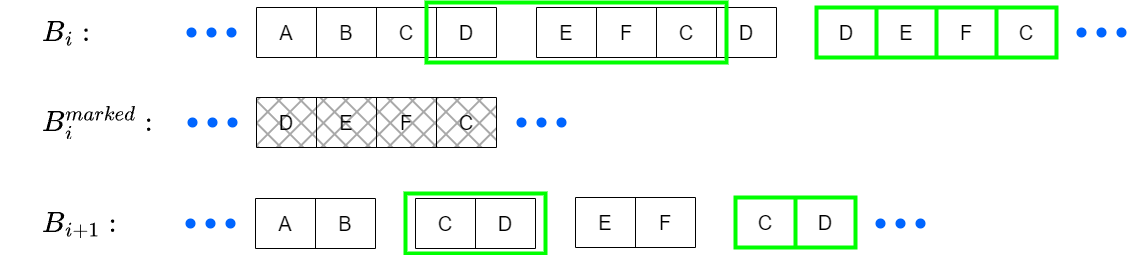
\includegraphics[width=1\textwidth]{Images/approxlz77.png}
    \caption{Die Abbildung illustriert die rundenbasierte Verarbeitung von Blöcken über der Eingabe in Approx. LZ77. In Runde $i$ werden die Blöcke in $B_i$ auf Referenzen untersucht und
    die Funde in die Menge der markierten Blöcke übernommen. Nur die unmarkierten Blöcke werden geteilt und in die nächste Runde übernommen.}
    \label{fig:roundapproxlz77}
\end{figure}
Innerhalb einer beliebigen Runde $i\int [1,log(|S|)]$ wird die Menge der Blöcke $B_i$ auf Referenzen, also auf vorherige Vorkommen in $S$, untersucht. Im Erfolgsfall wird für den Block und
dessen repräsentierter Zeichenfolge ein Faktor generiert. Weiterhin deklarieren wir den entsprechenden Block als markiert. Die Menge aller markierten Blöcke, die in der Runde $i$
erzeugt wurden, wird durch $B_i^{marked}$ mit $B_i^{marked}\subset B_i$ bezeichnet. Die verbleibenden Blöcke, $B_i^{unmarked}=B_i\setminus B_i^{marked}$, werden im Übergang
zur nächsten Runde jeweils gespaltet. Im Anschluss an die letzte Runde werden die repräsentierten Zeichen der unmarkierten Blöcke referenzlos interpretiert und faktorisiert.

In \ref{fig:roundapproxlz77} wird der Übergang zwischen zwei sukzessiven Runden an einem Beispiel verdeutlicht. Im Folgenden widmen wir uns einer algorithmischen Realisierung der beschriebenen
Methodik. Insbesondere wird die Extraktion von Referenzen in jeder Runde konkret thematisiert.
In \ref{alg:compapproxlz77} werden die notwendingen Prozesse vor, während und nach der rundenbasierten Ausführungsschleife von Approx. LZ77 beschrieben. Zu Beginn der initialen
Runde $r_{init}=1$ wird die gesamte Eingabe in $2^{r_{init}}$ Blöcke gleicher Größe eingeteilt. Dieser Prozess wird durch die Routine InitBlocks erfasst. Darauf folgt eine Schleife
über eine beschränkte Anzahl an Runden, die durch $r_{end}=log_2(|S|)$ definiert ist. Die Routine ProcessRound beschreibt die bereits erwähnte Extraktion von Referenzen über die
Menge der Blöcke, die eine Menge von markierten Blöcken und den zugehörigen Faktoren generiert. Im Übergang zur nächsten Runde werden die unmarkierten Blöcke in der Routine 
NextNodes jeweils gespaltet. Nach einer abschließenden Verarbeitung von referenzlosen Zeichen steht die Faktorfolge $F$ bereit.

\begin{algorithm}[ht]
\centering
\caption{COMP$_{ApproxLZ77}$: Approximation der exakten LZ77-Faktorisierung durch eine blockweise Referenzsuche} \label{alg:compapproxlz77}
\algorithmicrequire $S=e_1...e_n$
\algorithmicensure $F=f_1...f_z$
\begin{algorithmic}[1]
    \STATE $F \gets \emptyset$
    \STATE $r_{init} \gets 1$
    \STATE $r_{end} \gets log_2(|S|)$
    \STATE $Blocks[1..2^{r_{init}}] \gets InitBlocks(S, 2^{r_{init}})$ \algorithmiccomment{Split S into $2^{r_{init}}$ equal blocks}
    \FOR{$r \gets r_{init}$ \TO $r_{end}$}
        \STATE $markedBlocks[1..z_r] \gets ProcessRound(r, S, Blocks, F)$
        \STATE $Blocks \gets NextNodes(Blocks\setminus markedBlock[1..z_r])$ \algorithmiccomment{Halve unmarked blocks}
    \ENDFOR
    \FOR{$e \in Blocks$} 
        \STATE $F \gets F.insert(0, e)$ \algorithmiccomment{Process remaining Characters}
    \ENDFOR
    \RETURN $F$
\end{algorithmic}
\end{algorithm}

Die Funktionsweise der ProcessRound-Routine wird in \ref{alg:processround} beschrieben. Die Ausführung kann in drei Schritte unterteilt werden. Im ersten Schritt werden die Tabellen RFPTable und RefTable
mithilfe der Routine InitTables initialisiert. Die RFPTable ordnet jedem Rabin-Karp-Fingerprint(RFP), der über die Menge aller Blöcke berechnet wird, den linkesten Block zu, welcher diesen 
Wert ebenfalls aufweist. In diesem Rahmen vernachlässigen wir explizit Kollisionsfälle des RFP und gehen davon aus, dass die Gleichheit der RFPs zweier Zeichenfolgen ebenfalls die Gleichheit der Zeichenfolgen
impliziert. Die RefTable speichert für jeden Block die Position des linkesten Vorkommens, also einer Referenz, seiner Zeichenfolge in der Eingabe, die zum aktuellen Zeitpunkt bekannt ist.

\begin{algorithm}[ht]
    \centering
    \caption{ProcessRound: Jede Runde enkapsuliert die Referenzsuche unter allen Blöcken und innerhalb der Eingabe.} \label{alg:processround}
    \algorithmicrequire $r, S, Blocks$
    \algorithmicensure $markedBlocks$
    \begin{algorithmic}[1]
        \STATE $(RFPTable, RefTable) \gets InitTables(Blocks)$
        \STATE $ReferenceScan(S, Blocks, RFPTable, RefTable)$
        \FOR {$i \gets 1$ \TO $|Blocks|$}
            \IF{$RefTable[i] < Blocks[i].Pos$}
                \STATE $markedBlocks.insert(i)$
                \STATE $F.insert(\frac{|S|}{2^r}, RefTable[i])$ \algorithmiccomment{Ordered Insert}
            \ENDIF
        \ENDFOR
        \RETURN $markedBlocks$
    \end{algorithmic}
\end{algorithm}

Die Routine InitTables, wie in \ref{alg:inittables} beschrieben, erzeugt die RFPTable, indem alle Blöcke von links nach rechts durchlaufen werden und das Paar aus einem Block und dessen RFP in die Tabelle
nur dann eingefügt wird, wenn der RFP noch nicht vorhanden ist. Als Konsequenz wird für jeden RFP, der mindestens einem Block zugeordnet werden kann, der entsprechende linkeste Block gespeichert. Die RefTable
wird im gleichen Ablauf erzeugt. Falls der RFP eines Blocks bereits in der RFPTable vorhanden ist, so stellt der zugehörige Blockeintrag eine Referenz dar. In diesem Fall wird die Position des eingetragenen Blocks
in der RefTable eingetragen. Andernfalls ist der Block selbst das linkeste Vorkommen seiner Zeichenfolge, sodass die eigene Position eingetragen wird. Es ist zu betonen, dass die InitTables-Routine durch ihre 
Aktualisierungen der RefTable bereits markierte Blöcke bzw. Faktoren implizit erzeugt.

\begin{algorithm}[ht]
    \centering
    \caption{InitTables: Initialisierung der RFPTable und RefTable durch einen Scan der RFPs aller Blöcke} \label{alg:inittables}
    \algorithmicrequire $Blocks$
    \algorithmicensure $RFPTable, RefTable$
    \begin{algorithmic}[1]
        \STATE $RFPTable \gets HashTable[RFP, LeftMostBlock]$
        \STATE $RefTable[1..|S|] \gets (0,...,0)$
        \FOR{$i \gets 1$ \TO $|Blocks|$}
            \STATE $RFP \gets RFP(Blocks[i])$
            \IF{$RFP \textbf{ in } RFPTable$}
                \STATE $RefTable[i] \gets RFPTable[RFP].Pos$
            \ELSE
                \STATE $RFPTable.insert(RFP,Blocks[i])$
                \STATE $RefTable[i] \gets Blocks[i].Pos$
            \ENDIF
        \ENDFOR
        \RETURN $RFPTable, RefTable$
    \end{algorithmic}
\end{algorithm}

Im zweiten Schritt, dem RefereneScan \ref{alg:refscan}, werden zusätzliche Referenzen innerhalb der gesamten Eingabe $S$ gesucht. In einer beliebigen Runde $r$ wird der RFP eines Fensters der Größe $\frac{|S|}{2^r}$ 
über der Eingabe berechnet und mit den Einträgen der RFPTable verglichen. Im Falle eines Treffers wird die Position des Fensters in der RefTable eingetragen, falls er den vorherigen Wert unterbietet. Die Berechnung
des RFP des Fensters in Folge der sukzessiven Verschiebung um eine Position kann wie in \ref{eq:shift} beschrieben in konstanter Zeit durchgeführt werden.
Schließlich wird im dritten Schritt die RefTable genutzt, um die implizit markierten Blöcke zu extrahieren. Ein Block wird markiert, wenn die RefTable die Position einer Referenz indiziert, die kleiner als die
des Blocks ist. Die Position der Referenz und die rundenbedingte Blockgröße als Faktorlänge definieren einen eindeutigen Faktor, der in die Menge der Faktoren $F$ eingefügt wird. Die Reihenfolge der Faktoren
wird endgültig durch die Position der repräsentierten Zeichenfolge bestimmt. Für die Einhaltung der Reihenfolge sei im Rahmen der Analyse der Laufzeit und des Speicherverbrauchs eine nachträgliche Sortierung
der Faktoren in $F$ vorgegeben werden.

\begin{algorithm}[ht]
\centering
\caption{ReferenceScan: Suche zusätzliche Referenzen durch einen Scan der gesamten Eingabe} \label{alg:refscan}
\algorithmicrequire $S, Blocks, RFPTable, RefTable$
\begin{algorithmic} [1]
    \STATE blockSize $\gets \frac{|S|}{|Blocks|}$
    \STATE $RFP \gets RFP(S[1..blockSize])$
    \FOR{$i \gets 1$ \TO $|S|-blockSize$}
        \IF{$RFP \text{ in } RFPTable$ \AND $i < RefTable[RFPTable[RFP]]$}
            \STATE $RefTable[RFPTable[RFP]] \gets i$
        \ENDIF
        \STATE $RFP \gets RFP(S[i+1..i+blockSize])$ \algorithmiccomment{Rolling Hash}
    \ENDFOR
\end{algorithmic}
\end{algorithm}


\subsection{Theoretisches Laufzeit- und Speicherverhalten}
Die Laufzeit des Algorithmus wird durch die Anzahl der Runden und der Extraktion von Referenzen in jeder Runde bestimmt. Die Anzahl der Runden beträgt maximal $log_2(|S|)=log_2(n)$. In jeder Runde
werden Referenzen unter den Blöcken durch die InitTables-Routine bestimmt. Die Menge aller Blöcke, die in dieser Routine bearbeitet werden, decken maximal die gesamte Eingabe $S$ ab. Die Laufzeit
der Routine erhält durch die Berechnung des RFPs über dieser Zeichenfolge eine Laufzeitschätzung von $O(n)$. Die Referenzsuche über die gesamte Eingabe durch die ReferenceScan-Routine benötigt ebenfalls
$O(n)$ Laufzeit, da das berücksichtigte Fenster in linearer Zeit über die Eingabe verschoben werden kann. Durch die Verwendung einer Hashtabelle sind die Suchoperationen jeweils in konstanter Zeit
durchführbar. Die Laufzeit der ProcessRound-Routine beträgt somit $O(n)$. Insgesamt ergibt sich eine Gesamtlaufzeit von $O(n\log{n})$ für Approx. LZ77. 
Der Speicherbedarf des Algorithmus wird durch die Größe der Blockmenge,RFPTable und der RefTable bestimmt, die wiederum alle durch die Anzahl der Blöcke bestimmt werden. In jeder Runde repräsentiert 
die Menge der Blöcke die noch unverarbeitete Eingabe, sodass aus jedem Block im Laufe des Algorithmus mindestens ein Faktor extrahiert wird. Die Anzahl der Blöcke einer Runde übersteigt damit nie die 
Größe der endgültigen Faktorfolge, $|F|=z$. Der Speicherbedarf kann damit konservativ auf $O(z)$ abgeschätzt werden.

\section{Parallelisierung von Approx. LZ77(Approx. LZ77Par)}
\subsection{Konzept}
Im Folgenden beschreiben wir die verwendete Methodik zur Parallelisierung von Approx. LZ77. Die parallele Variante des Algorithmus, die wir Approx. LZ77Par nennen, basiert auf der abgeschlossenen
Parallelisierung von Abschnitten von Approx. LZ77, die eine chronologische Abhängigkeit aufweisen. Für die Parallelisierung der Verarbeitung wird jeweils die Eingabe auf verschiedene Prozessoren 
bzw. Threads verteilt und ein gemeinsames Ergebnis erzeugt.
\begin{figure}[ht]
    \centering
    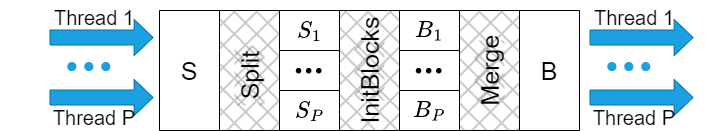
\includegraphics[width=0.8\textwidth]{Images/parallel_initnodes.png}
    \caption{Parallele Generierung der initialen Blöcke}
    \label{fig:parinitnodes}
\end{figure}
In \ref{fig:parinitnodes} wird die parallele Generierung der initialen Blöcke dargestellt. Hierbei wird die Eingabe $S$ in $P$ Teile aufgebrochen, sodass die Routine InitBlocks auf jedem Prozessor
die zugehörigen Blöcke erzeugen kann. Da die Ordnung und die Größe der Ergebnisse bekannt ist, kann eine umfassende Blockmenge ohne zusätzlichen Aufwand erzeugt werden.
\begin{figure}[ht]
    \centering
    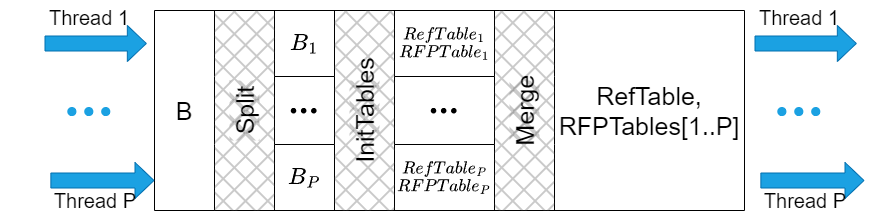
\includegraphics[width=0.8\textwidth]{Images/parallel_inittables.png}
    \caption{Parallele Initialisierung der RFP-Tabelle und der Referenztabelle}
    \label{fig:parinittables}
\end{figure}
In \ref{fig:parinittables} wird die parallele Initialisierung der RFPTable und der RefTebl dargestellt. Die Menge aller Blöcke wird in $P$ Teile aufgeteilt, wobei als Kriterium für die
Aufteilung der RFP jedes Blocks verwendet wird. Als Konsequenz werden identische Zeichenfolgen nicht auf verschiedene Prozessoren verteilt. Jeder Prozessor erzeugt eine eigene RFPTable, wobei
die RefTable durch alle Prozessoren gemeinsam aktualisiert wird. Auch hier wird durch den RFP als Aufteilungsschlüssel eine Überlappung der Zugriffe vermieden. Das Ergebnis ist eine konsistente
RefTable und eine $P$-elementige Menge von Instanzen der RFPTable, die jeweils eine klar abgegrenzte Teilmenge aller RFPs abdecken.

\begin{figure}[ht]
    \centering
    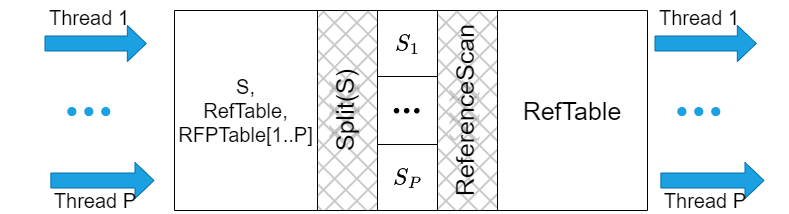
\includegraphics[width=0.8\textwidth]{Images/parallel_referencescan.png}
    \caption{Paralleler Scan der Eingabe nach zusätzlichen Referenzen}
    \label{fig:parrefscan}
\end{figure}
In \ref{fig:parrefscan} wird der parallele Scan der Eingabe $S$ nach zusätzlichen Referenzen dargestellt. Die Eingabe $S$ wird in $P$ Teile aufgeteilt. Auf jede Teilfolge wird die sequenzielle Routine
ReferenceScan angewendet, wobei die RefTable durch alle Prozessoren gemeinsam aktualisiert wird und ein potenziell paralleler Lesezugriff auf Instanzen der RFPTable stattfindet. 
Schließlich müssen die implizit erzeugten Faktoren in die Menge der Faktoren $F$ eingefügt werden. Da die Reihenfolge der Faktoren erhalten bleiben muss, wird eine nachträgliche parallele Sortierung
verwendet. Die Implementierung der parallelen Sortierung ist jedoch nicht Gegenstand dieser konzeptuellen Analyse und wird daher nicht weiter betrachtet. Eine mögliche Implementierung ist in (\cite{parallelcomputing}) 
beschrieben.

\subsection{Theoretisches Laufzeit- und Speicherverhalten}
Da die Eingabe stets in gleiche Teile aufgeteilt und die Ausgabe ohne einen relevanten Aufwand kombiniert werden kann, kann eine theoretische Laufzeit von $O(\frac{n \log n}{P})$ geschätzt werden, 
wobei $P$ die Anzahl der Prozessoren definiert. Der Speicherbedarf des Algorithmus beträgt weiterhin $O(z)$. Dies stellt jedoch eine
ideale Abschätzung dar, die in der Praxis nicht erreicht werden kann. Insbesondere die Interaktion mit dem Speicher und die Kommunikation zwischen den Prozessoren führen zu einer oberen Schranke
des Speedups.

\section{Praktische Optimierungen} \label{sec:practopt}
Im Folgenden betrachten wir optionale Optimierungen, die die durchschnittliche Laufzeit von Approx.LZ77 und Approx.LZ77Par verbessern können auf Kosten von anderen Metriken. Jede einzelne Technik
ist optional und unabhängig von den Anderen nutzbar, wobei eine positive Korrelation zu erwarten ist.

\subsection{Dynamische Endrunde(DynEnd) - Laufzeit vs. Qualität*}
Sei eine beliebige lineare Kodierung $K_{OUT}$ für die Übersetzung der erzeugten Faktorenfolge $F$ gegeben. Der Wert,
\begin{equation}
    Min^{Ref}_{Bin}=min\{|K_{OUT}(f)| | f \in F ,f \text{ ist Referenz}\}
\end{equation}
gibt die minimale Anzahl an Bits an, die für die Kodierung einer beliebigen Referenz benötigt wird. Analog dazu beschreibt
\begin{equation}
    Max^{Lit}_{Bin}=max\{|K_{OUT}(f)| | f \in F, f \text{ ist Zeichen}\}
\end{equation}
die maximale Anzahl an Bits, die für die Kodierung eines referenzlosen Zeichens benötigt wird. Sei $f_{ref}$ ein beliebiger referenzierender Faktor, welcher 
$|f_{ref}|\leq\frac{Min^{Ref}_{Bin}}{Max^{Lit}_{Bin}}$ Zeichen referenziert. Die referenzierte Zeichenfolge von $f_{ref}$ wird im Folgenden als $S_{ref}$ mit $|S_{ref}|=|f_{ref}|$ bezeichnet.
Dann gilt für die Länge der kodierten Repräsentation von $f_{ref}$:
\begin{equation}
\begin{split}
    |K_{OUT}(f_{ref})| & \geq Min^{Ref}_{Bin}\\
    & \geq |f_{ref}| \cdot Max^{Lit}_{Bin}\\
    & \geq \sum_{i=1}^{|f_{ref}|} |K((0, S_{ref}[i]))|.
\end{split}
\end{equation}
Es folgt, dass ein referenzierender Faktor, dessen Länge eine obere Schranke von $\frac{Min^{Ref}_{Bin}}{Max^{Lit}_{Bin}}$ Zeichen nicht überschreitet, nicht effizient kodiert werden kann.
Stattdessen sollten die referenzierten Zeichen einzeln kodiert werden. Die Technik der dynamischen Endrunde greift diese Idee auf, indem Referenzen unterhalb einer Grenzlänge nicht extrahiert
werden. Gibt uns die Kodierung eine Grenzlänge $l^{ref}_{min} = \lceil\frac{Min^{Ref}_{Bin}}{Max^{Lit}_{Bin}}\rceil$ vor, so kann der Algorithmus in Runde 
$r_{DynDnd} = \lceil log_2{|S|}-log_2{l^{ref}_{min}} \rceil$ terminieren. Da potenziell referenzierende Faktoren aufgebrochen werden, kann die Qualität der Faktorisierung sinken, wobei das 
binäre Endprodukt kleiner wird. Es ergibt sich also eine steigende Faktorrate bei einer gleichzeitig sinkenden Kompressionsrate.
\begin{equation}
    CR^{Approx.LZ77}_{DynEnd} \leq CR^{Approx.LZ77}
\end{equation}
\begin{equation}
    FR^{Approx.LZ77}_{DynEnd} \geq FR^{Approx.LZ77}
\end{equation}

\subsection{Dynamische Startrunde(DynStart) - Laufzeit vs. Speicher} \label{sec:dynstart}
Gegeben seien zwei initiale Runden $r_{init1}$ und $r_{init2}$ mit $1\leq r_{init1} < r_{init2}\leq log_2{|S|}$, die auf der gesamten Eingabe S angewendet werden, 
so wird die Eingabe jeweils in $2^{r_{init1}}$ bzw. $2^{r_{init2}}$ Blöcke gleicher Größe eingeteilt. Die Mengen der Blöcke werden im Folgenden als $B_{init1}$ bzw. $B_{init2}$ bezeichnet.
Im Rahmen der Bearbeitung der Runden wird eine Menge von markierten Blöcken $B_{init1}^{marked}\subset B_{init1}$ bzw. $B_{init2}^{marked}\subset B_{init2}$ erzeugt, für die ein vorheriges
Vorkommen bestimmt wurde. Aufgrund der Natur der Blockspaltung in jeder Runde, kann jedem Block in $B_{init1}$ eine Gruppe von $2^{r_{init2}-r_{init1}}$ Blöcken in $B_{init2}$ zugeordnet
werden, die die gleiche Zeichenfolge repräsentieren. Die Folgerung lässt sich insbesonere auch auf die markierten Blöcke anwenden, sodass die folgende Beziehung hergeleitet werden kann:
\begin{equation}
    |B_{init2}^{marked}| \geq 2^{r_{init2}-r_{init1}} \cdot |B_{init1}^{marked}|.
\end{equation}
Weiterhin folgt, dass die Existenz eines markierten Blocks in $B^{init1}$ die Existenz von $2^{r_{init2}-r_{init1}}$ benachbarten markierten Blöcken in $B^{init2}$ impliziert. Die
Umkehrung dieser Aussage liefert,
\begin{equation}
    longestChain(B_{init2}^{marked}) < 2^{r_{init2}-r_{init1}} \Rightarrow B_{init1}^{marked}=\emptyset, 
\end{equation}
wobei $longestChain(B^{init2}_{marked})$ die Größe der längsten Kette von benachbarten markierten Blöcken in $B_{init2}^{marked}$ bezeichnet.
Die Technik der dynamischen Startrunde greift diese Beziehung auf, indem initial die Runde $r_{init}=log_2{|S|}/2$ auf die gesamte Eingabe S angewendet wird. Im Anschluss
kann der Wert $longestChain(B_{init}^{marked})$ mithilfe eines Scans über die markierten Blöcke bestimmt werden. Der errechnete Wert impliziert eine Runde $r_{DynStart}$ derart,
dass vorherige Runden garantiert keine markierten Blöcke erzeugen und damit ausgelassen werden können. Der Wert $r_{DynStart}$ ergibt sich wie folgt,
\begin{equation}
    r_{DynStart} = r_{init}-
    \begin{cases}
        -1, & \text{falls } longestChain(B^{init}_{marked}) = 0\\
        \lfloor log_2{longestChain(B^{init}_{marked})} \rfloor, & \text{sonst}
    \end{cases}
\end{equation}
In Abhängigkeit von der Beschaffenheit der Eingabe, kann maximal die Hälfte aller Runden ausgelassen werden, ohne eine Veränderung der Ergebnisse zu verursachen. In
Runde $r_{init}=log_2{|S|}/2$ werden jedoch $2^{log_2{|S|}/2}=\sqrt{|S|}$ Blöcke erzeugt. Dies führt zu einer zusätzlichen unteren Schranke für den Speicheraufwand des Algorithmus.
Falls diese Technik angewandt wird, kann der Speicheraufwand mit $O(\max\{\sqrt{n}, z\})$ abgeschätzt werden.

\subsection{Vorberechnete Runde(PreMatching) - Laufzeit vs. Speicher}
Analog zu der dynamischen Startrunde kann eine vorberechnete Runde ebenfalls genutzt werden, um den Arbeitsaufwand vorheriger Runden zu reduzieren. Sei $r_{PreMatch}$ mit 
$1\leq r_{PreMatch} \leq log_2{|S|}$ eine Runde, die auf die gesamte Eingabe angewendet wird. Als Ergebnis erhalten wir die Menge der markierten Blöcke, $B_{PreMatch}^{marked}$.
Weiterhin speichern wir uns die RFPs aller Blöcke, die im Rahmen der Runde generiert wurden. Wie in \ref{sec:dynstart} gezeigt, kann jedem Block in einer vorherigen Runde einer Gruppe
von Blöcken in einer späteren Runde zugeordnet werden, die die gleiche Zeichenfolge repräsentieren. Die Konkatenation von Zeichenfolgen kann in Anlehnung an \ref{eq:concat} auf eine
Operation auf der Basis des RFP abgebildet werden. Gegeben sei eine Runde $r_m$ mit $1\leq r_m \leq r_{PreMatch}$. Für einen beliebigen Block $b \in B_m$ können 
$2^{r_{PreMatch}-r_m}$ viele Böcke $(b_1, b_2, ..., b_{2^{r_{PreMatch}-r_m}})\in B_{prematch}$ gefunden werden, deren Konkatenation die gleiche Zeichenfolge repräsentieren. So ergibt sich 
für den zugehörigen RFP,
\begin{equation}
    RFP(b) = RFP(b_1 \cdot b_2 \cdot ... \cdot b_{2^{r_{PreMatch}-r_m}}),
\end{equation}
wobei jede Konkatenation in eine Operation mit konstanter Laufeit für die RFPs abgebildet werden kann. Die Anzahl der Rechenschritte für die Berechnung des RFP eines Blockes hängt nun 
nicht mehr von der Länge der repräsentierten Zeichenfolge sondern der Rundendistanz zur vorberechneten Runde ab.
Weiterhin kann die Menge der unmarkierten Blöcke $B_{PreMatch}^{unmarked}=B_{PreMatch}\setminus B_{PreMatch}^{marked}$ genutzt werden, um die Menge der Blöcke $B_m$ in Runde $r_m$
zu filtern. Sei ein Block $b \in B_m^{marked}$ gegeben, so muss die equivalente Sequenz von Blöcken $(b_1, b_2, ..., b_{2^{r_{PreMatch}-r_m}})\in B_{prematch}$ auch markiert sein bzw.
Teil von $B_{prematch}^{marked}$ sein.
Die Umkehrung dieser Aussage liefert einen Filter für alle vorherigen Runden, um Blöcke auszugrenzen, die keine Kandidaten für eine Markierung sind. Die zusätzlich gespeicherten Daten 
erhöhen den Speicherbedarf des Algorithmus. 
Sei $r_{PreMatch}\in [1, log_2{|S|}]$ der Index der vorberechneten Runde, so kann der resultierende Speicherbedarf mit $O(\max\{2^{r_{PreMatch}}, z\})$ abgeschätzt werden.

\subsection{Minimale Tabellengröße(ScanSkip) - Laufzeit vs. Qualität}
Wie in \ref{alg:inittables} beschrieben, wird die RFPTable und die RefTable durch die InitTables-Routine initialisiert. Im Rahmen der Routine werden alle Blöcke auf Duplikate
überprüft, sodass nur einzigartige Blöcke in die RFPTable eingefügt werden und die RefTable resultierende implizite Faktoren speichert. Die Anzahl der Blöcke, die im nachfolgenden Schritt 
in der ReferenceScan-Routine \ref{alg:refscan} markiert werden können, ist durch die Anzahl der Einträge in der RFPTable beschränkt. Der Wert $k\in [0,1]$ gebe den Anteil der
Einträge in der RFPTable in Relation zur Gesamtzahl der Blöcke an. Unsere Optimierung sieht vor, dass in jeder Runde die ReferenceScan-Routine nur angewendet wird, falls $k$ größer
als ein Schwellwert $k_{min}\in [0,1]$ ist. Faktoren, die durch die ausgelassene Suche in dieser Runde nicht erzeugt wurden, werden in einer der nächsten Runden ausgegeben, wobei diese
durch die Halbierung der Blöcke sukzessive in ihrer Anzahl verdoppelt werden. Damit steigt zwangsläufig die Faktorrate, wobei die ausgelassene Referenzsuche einen zeitlichen Gewinn bringt.
Es wurde bereits etabliert, dass die Anzahl der Blöcke in jeder Runde durch die Anzahl der Faktoren, $z$, beschränkt ist. Die Anzahl der Faktoren, die durch die Auslassung von 
ReferenceScan in einer Runde nicht erzeugt werden, ist durch $k_{min} \cdot z$ beschränkt. Ähnlich dazu ist die Anzahl der zusätzlich erzeugten Faktoren in der nächsten Ausführung
der Referencescan-Routine durch $2 \cdot k_{min} \cdot z$ beschränkt. Die Häufigkeit dieser Ereigniskette hängt von der Beschaffenheit der Eingabe ab, wobei die Anzahl der
Runden als konservative obere Schranke genutzt werden kann. Insgesamt ergibt sich eine konservative obere Schranke für die relative Verschlechterung der Faktorrate um den Faktor 
$(1 + k_{min} \cdot {log_2{|S|}})$.

\subsection{Korrelation der Optimierungen}
Die Einschränkung der initialen und terminalen Runde durch DynStart und DynEnd reduziert die potenzielle Rundendistanz zu einer gewählten vorberechneten Runde, $r_{PreMatch}$.
Dies unterstützt die zeitsparende Wirkung von PreMatching. Die Filterung von Blöcken, die keine Kandidaten eine Markierung sind, durch PreMatching erlaubt eine Reduktion der 
RFPTable, die durch die InitTables-Routine erzeugt wird. Entsprechend kann für die ScanSkip-Optimierung ein kleinerer Wert für $k_{min}$ gewählt werden, um die Verschlechterung
der Faktorrate bei gleicher Häufigkeit der ausgelassenen ReferenceScan-Routine zu reduzieren. Diese Überlegungen stellen eine zu erwartende Korrelation der Optimierungen dar,
wobei die spezifischen Auswirkungen von der Beschaffenheit der Eingabe und der Wahl der Parameter abhängen.